\documentclass[fleqn, 10pt]{article}

\usepackage[utf8]{inputenc}
\usepackage[spanish]{babel}
\usepackage{amsthm}
\usepackage{nccmath}
\usepackage{enumitem}
\usepackage{graphicx}
\usepackage{verbatim}
\usepackage{algpseudocode}



\theoremstyle{plain}
\newtheorem{proposicion}{Proposición}

\theoremstyle{definition}
\newtheorem{definition}{Definición}[section]
\newtheorem{example}{Ejemplo}[section]


\title{Teoría de Autómatas y Lenguajes Formales\\[.4\baselineskip]Práctica 4.}
\author{Carlos Velasco Hilario}
\date{24/12/2022}


\begin{document}

\maketitle

\section{Create the simplest WHILE program that computes the diverge function and compute the codification of its code. }

\begin{verbatim}
                     Q = (0,s)
                       s:
                         X1 := X1 + 1;
                         while X1 != 0 do
                          X1 := X1
                         od
\end{verbatim}
La primera instruccion es la mas importante para asegurarnos de que el programa siempre diverje. Para esto, nos aseguramos de utilizar un bucle con el minimo cuerpo posible.


\begin{center}
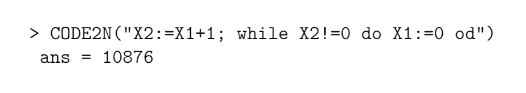
\includegraphics[width=11cm, height=2cm]{codigoej1p4.png}
\end{center}
\newpage

\section {Create an Octave script that enumerates all the vectors.}
\begin{verbatim}

function printNvectors(N)
for i=0:N-1
disp([’(’ num2str(godeldecoding(i)) ’)’])
end
end


\end{verbatim}
\begin{center}
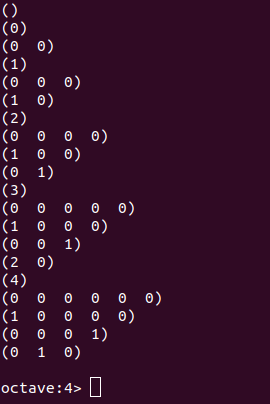
\includegraphics[width=5cm, height=8cm]{ejercicio2p4.png}
\end{center}

\begin{center}
\end{center}

\newpage
\section {Create an Octave script that enumerates all the WHILE programs.}
\begin{verbatim}
function printNwhilePrograms(N)
for i=0:N-1
disp(N2WHILE(i))
end
end

\end{verbatim}
\begin{center}
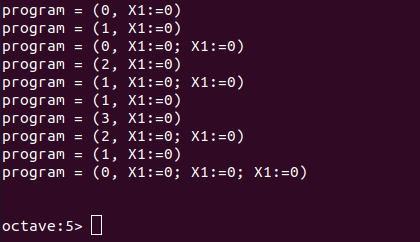
\includegraphics[width=9cm, height=6cm]{ejercicio3p4.png}
\end{center}
\end{document}